Implementation chapter is meant to cover the actual experimentation and programming part of this thesis. Reader of this document is lead through series of experiments and examples and is taken on journey to a reliable solution of the matter. On following pages you will find and reveal complexity of this problem.

This chapter aims to show and uncover every detail the author stumbled upon when he tried to implement the solutions proposed by Hinton\,\cite{capsule}, which we elaborated in detail in Chapter \ref{chapter:research}. Moreover we will discuss the differences when this solution is compared to other, related implementations mentioned in the Chapter \ref{chapter:solutions}.

\section{Preparation and prerequisites}

\textit{Keras} with \textit{TensorFlow} back-end was selected as the key framework to use for this implementation. That inherently means, we are bound to use Python as a programming language. However, selection of Python is natural and reasonable anyways, since it is the most used language in the field of machine learning, artificial intelligence experimentation. Moreover due to technical limitation and proven better performance, Anacoda Python distribution is selected as the proper back-end. According to various researches\,\todo{cite} and projects, \textit{TensorFlow} performance fluctuates a lot since the pre-compiled packages are not allowed to use all the capabilities of each and every specific hardware combination. Therefore projects like Thoth\footnote{http://thoth-station.ninja} were created to provide dependency mesh mapping . In our example we can be satisfied by the enhanced performance of Anaconda/Conda \textit{TensorFlow} distribution (from either Anaconda or Intel channels). Moreover, running \textit{TensorFlow} locally on CPU is used for quick prototyping. For more demanding executions, Google Colab\footnote{https://colab.research.google.com} is selected as Jupyter notebook execution provider. All source codes to this implementation were released under Apache 2.0 license on Git Hub\footnote{https://github.com/tumido/capsnet-face}.

\section{Keras on TensorFlow}

\textit{Keras} is a high level API for machine learning. It provides unified means to define and access models and layers as well as most common mathematical principles and functions in a highly polished package. This package relies on a back-end provider to implement the solutions behind the scenes. \textit{TensorFlow} is one of these back-end. Principles of this cooperation and more elaborate description of other back-ends and solutions can be found in chapter \ref{chapter:solutions}.

Let's provide a basic overview of the available API and bindings that will be used later on in our implementation:

\begin{lstlisting}[language=Python, caption=Keras example]
from keras import models, layers

# Procedural model declaration
model = models.Sequential(
    name="sequential_model",
    layers=[
        layers.Dense(...),
        layers.Conv2D(...),
        ...
    ]
)

# Functional model definition
input_layer = layers.Input(shape=(...))
output = layers.Dense(...)(input_layer)
output = layers.Conv2D(...)(output)
...
final_layer = layers.Conv2D(...)(output)

model = models.Model(
    name="raw_model",
    inputs=[x]
    outputs=[final_layer]
)
\end{lstlisting}

As you can see using \textit{Keras} is straightforward. It allows an easy model definition using various approaches. This provides a great benefit, which we will use later on\,--\,it allows model stacking, permutation of layers, combination of layouts while easily sharing parameters and behaviour. This gives the researcher a really powerful mean to manipulate a model and shape it to achieve desired behaviour, even multiple distinct behaviours for each phase of the model's life cycle. It allows easy way to inject or extract auxiliary inputs and outputs into the model configuration. This is a really important feature especially in our case, as you will learn later on next pages, since we desire a much different model behaviour when the network is trained to the one when we ask for a prediction.

In next few paragraphs we will show what network configuration we chose for our CapsNet as well as observe proven and experimental configurations of the layers involved. As you might know, layers are the basic building blocks of neural networks. And stacking these layers one on top of another creates more complex behaviours. Certain patterns of layers usually results into an architecture. Models can use a straight, classic scheme of layering one layer onto one another layer, or it can diverge at certain point and result into multiple behaviours. The first one uses \texttt{keras.models.Sequential} type of neural network. This means a single set of inputs is passed to the model, the model processes the data through each and every layer in the same order, and at the end, the last layer in the sequence, produces the desired output. The later mentioned behaviour, required more complex yet precise handling. This allows the researcher much greater control over what inputs are passed to which layer, and which outputs are collected. \textit{Keras} allows this type of modelling via \texttt{keras.models.Model} class.

Later on, we will find out that even combination of these methods are possible. This allows to inject and join models, reuse a model in multiple parts of the network and most importantly it allows sharing of trained parameters. In our case, we will later on describe \textit{Encoder} and \textit{Decoder} logic as separate models or network prototypes which are combined into a greater models for two distinct purposes, training the network and testing. The trained network has one configuration, while the model used for prediction consists of partially different layers. But since this reuse of network parts is possible, we can leverage the trained parameters from the training phase, and use them in a different network which provides predictions.

\subsection{Layers}

In next few paragraphs we will introduce all the layers used in our solution and get familiar with their respective API first before we start putting them together into an actual network model configuration. Just before we do that, let's describe the common API for all layers:

\begin{lstlisting}[language=Python, caption=Common layer API]
layers.Layer(
    name="layer_name",  # Allows to name layer for proper storing
    input_shape=,       # Required input shape
    output_shape=,      # Required output shape
    trainable=,         # Can make the layer static
    weights=,           # Preset weights
    ...
)
\end{lstlisting}

Most of the arguments above can be defined on the fly, omitted or abstracted. Except for one, which is really important to use, in case we desire to store the model for later use. And that's the \texttt{name} parameter. This string allows user to specify unique name within the architecture for this particular layer. And since we can share layers between models, this feature can be leveraged to load the proper weights data into a different model, despite being exported from another one. This topic will be covered more in the Section\,\ref{ss:save_model}.

\subsubsection{\texttt{keras.layers.Input}}

Fundamental layer which allows to pass input data to a model. This layer has the biggest say in the shape of consumed data.

\begin{lstlisting}[language=Python, caption=Input layer]
layers.Input(
    shape=input_shape  # A shape in a tuple format without
                       # the first batch_size dimension
)
\end{lstlisting}

\subsubsection{\texttt{keras.layers.Dense}}

A \textit{Dense} stands for a well known, fully connected neural networks layer. It's product can be represented as equation \ref{eq:dense}, where the \texttt{act} is an activation function. This activation is performed over a element-wise multiplication of the input and a weight matrix kernel with additional bias added. Both kernel and bias are learned through training.

\begin{equation}
    o_{ij} = act(i_{ij} \times k + b_{ij})
    \label{eq:dense}
\end{equation}

This layer provides more extensive API, but in our implementation we will be satisfied with the basics. The example calls for each layer in later text is used directly from our \textit{CapsNet} implementation.

\begin{lstlisting}[language=Python, caption=Dense layer]
layers.Dense(
    units=400,          # Sets dimensionality of the output
    activation='relu',  # Desired activation function
    input_dim=prediction_caps_dim * bins, # Input dimensionality
    ...
)
\end{lstlisting}

\subsubsection{\texttt{keras.layers.Conv2D}}

Provides a two dimensional convolution. Convolution as operation as well as its meanings were already described in Section\,\ref{ss:conv}. This layer type utilizes these principles in 2D space. \textit{Keras} provides also other layer types for 1D and 3D convolution. However, the matter of our use case lays in image processing. And since images are a spatial two dimensional space, it dictates the use of \texttt{keras.layers.Conv2D}. In \textit{Keras}, there are also other layers like \texttt{keras.layers.Convolution2D}, though this is just an alias which points to the same implementation as \texttt{keras.layers.Conv2D}.

\begin{lstlisting}[language=Python, caption=2D convolution layer]
layers.Conv2D(
    filters=init_conv_filters,     # Amount of filters
    kernel_size=init_conv_kernel,  # Specifies height and weight of
                                   # kernel matrix
    strides=1,                     # A number of strides to use
    padding='valid',               # Sets padding on outer borders
    activation='relu',             # Desired activation function
    ...
)
\end{lstlisting}

\subsubsection{\texttt{keras.layers.Dropout}}

An over-fit prevention layer, which randomly sets each particular input to 0 with probability of \texttt{rate}. This is performed on each update during the training phase.


\begin{lstlisting}[language=Python, caption=Dropout layer]
layers.Dropout(
    rate=.3  # Fraction of input to drop
    ...
)
\end{lstlisting}

\subsubsection{\texttt{keras.layers.Reshape}}

A simple layer which allows to modify the shape of the input data. The result shape consists of \texttt{batch\_size} as first dimension and \texttt{target\_shape} as the rest. A special value of $-1$ can be used, which is treated as a variable, calculated, dimension.

\begin{lstlisting}[language=Python, caption=Reshape layer]
layers.Reshape(
    target_shape=[-1, capsule_dim], # Desired shape on output
    ...
)
\end{lstlisting}

\subsubsection{\texttt{keras.layers.Lambda}}

This is the first more complex layer. it might not seem so, however this layer allows to add custom behaviour. Its name is derived from lambda function, anonymous functions which are invoked in situ. The \texttt{keras.layers.Lambda} layer allows user to invoke any operation and transformation defined as a function. We use this type of layer in multiple scenarios, but for clarity we will list here just a single one\,--\,a calculation of length of each vector in the tensor.

\begin{lstlisting}[language=Python, caption=Lambda layer]
def length(inputs):
    return k.sqrt(k.sum(k.square(inputs), axis=2))

layers.Lambda(
    length
    ...
)
\end{lstlisting}


\subsubsection{\texttt{keras.layers.Layer}}

This abstract class serves as a base for all standard as well as all any custom layers in \textit{Keras}. It's behaviour and shape is fully customizable. Inheritance from this class allows user to invent and define a brand new layer, while maintaining the same API and compilation strategy as for any standard layer. While this might sound confusing the authors of \textit{Keras} framework made it really easy to comprehend and straightforward to implement. Let's take a look:


\begin{lstlisting}[language=Python, caption=Custom layer example]
class PredictionCapsule(layers.Layer):
    def __init__(self, custom_arg, **kwargs):
        """Init takes all custom parameters required for the behavior."""
        self.custom_arg = custom_arg

        # Pass the standard params to base class
        super(PredictionCapsule, self).__init__(**kwargs)

    def get_config(self):
        """Configuration of layer, used when saving a model."""
        return dict(
            custom_arg=self.custom_arg,
            **super(PredictionCapsule, self).get_config()
        )

    def compute_output_shape(self, input):
        """Allows layer to tell output shape based on input."""
        return (None, self.custom_arg * 5)

    def build(self, input_shape):
        """Called when model is created, allows weights init."""
        assert len(input_shape) == 3, "Wrong shape"
        self.W = self.add_weight(
            shape=[1,2,3],
            name='W',
            trainable=True,
        )
        # Required to be called when done
        super(PredictionCapsule, self).build(input_shape)

    def call(self, inputs, **kwargs):
        """Custom behavior. Needs to return agreed output shape."""
        ...
        return outputs

\end{lstlisting}


\section{Architecture}

Now, when we understand what types of layer we have available, we can dive in and start building from these basic blocks a full \textit{CapsNet} network. As we've already discussed in the chapter \ref{chapter:research}, the base structure of a capsule network is not as complicated as a CNN would be, however it requires some additional, custom entities and treatment as well. Starting from the simple to the more difficult, we are about to discover the overall architecture first and granularly enhance and dig deep into detail later.

Overall, the architecture is straightforward, but for good results it requires to be build from two separate distinct units, which when combined can be successfully trained. As per Hinton \cite{capsule}, we'll use the same naming conventions:

\begin{enumerate}
    \item \textbf{Encoder} is the actual network of containing capsules. It serves for feature recognition and classification.
    \item \textbf{Decoder} on the other hand is a helping force in training. It tries to reconstruct the input image based on prediction provided by the encoder.
\end{enumerate}

Also, it's worth mentioning a \textit{CapsNet} is not a \textit{single-input, single-output} type of network. For training purposes, it consumes both the image and the label and outputs a predicted label along with a reconstructed image. This behavior changes when the network is used for predictions. At that point the neural network is expected to behave and process a single input image and provide one output for it\,--\,the predicted label. However more outputs might be required in inference, since instead of a prediction we can be more interested in a similarity vector, which might be a better fit for unknown identity description. One way or another, any of these scenarios requires a different model layout. And since it's not possible to achieve a multiple layouts with a single model, we're destined to use multiple models, each with different layer structure. So now, we need to make sure that once we train one model the other one is capable to benefit from it as well. And now it's the right time to use the layer sharing between models as described above.

\section{Encoder}

Encoder serves as the true capsule network. It is expected to consume an image containing a face and to produce a prediction of an identity the input belongs to. This is achieved by a series of layers as described in the chapter \ref{chapter:research}. The structure prescribed by the following image is then implemented using layers described in this chapter.

\begin{figure}[ht!]
    \centering
    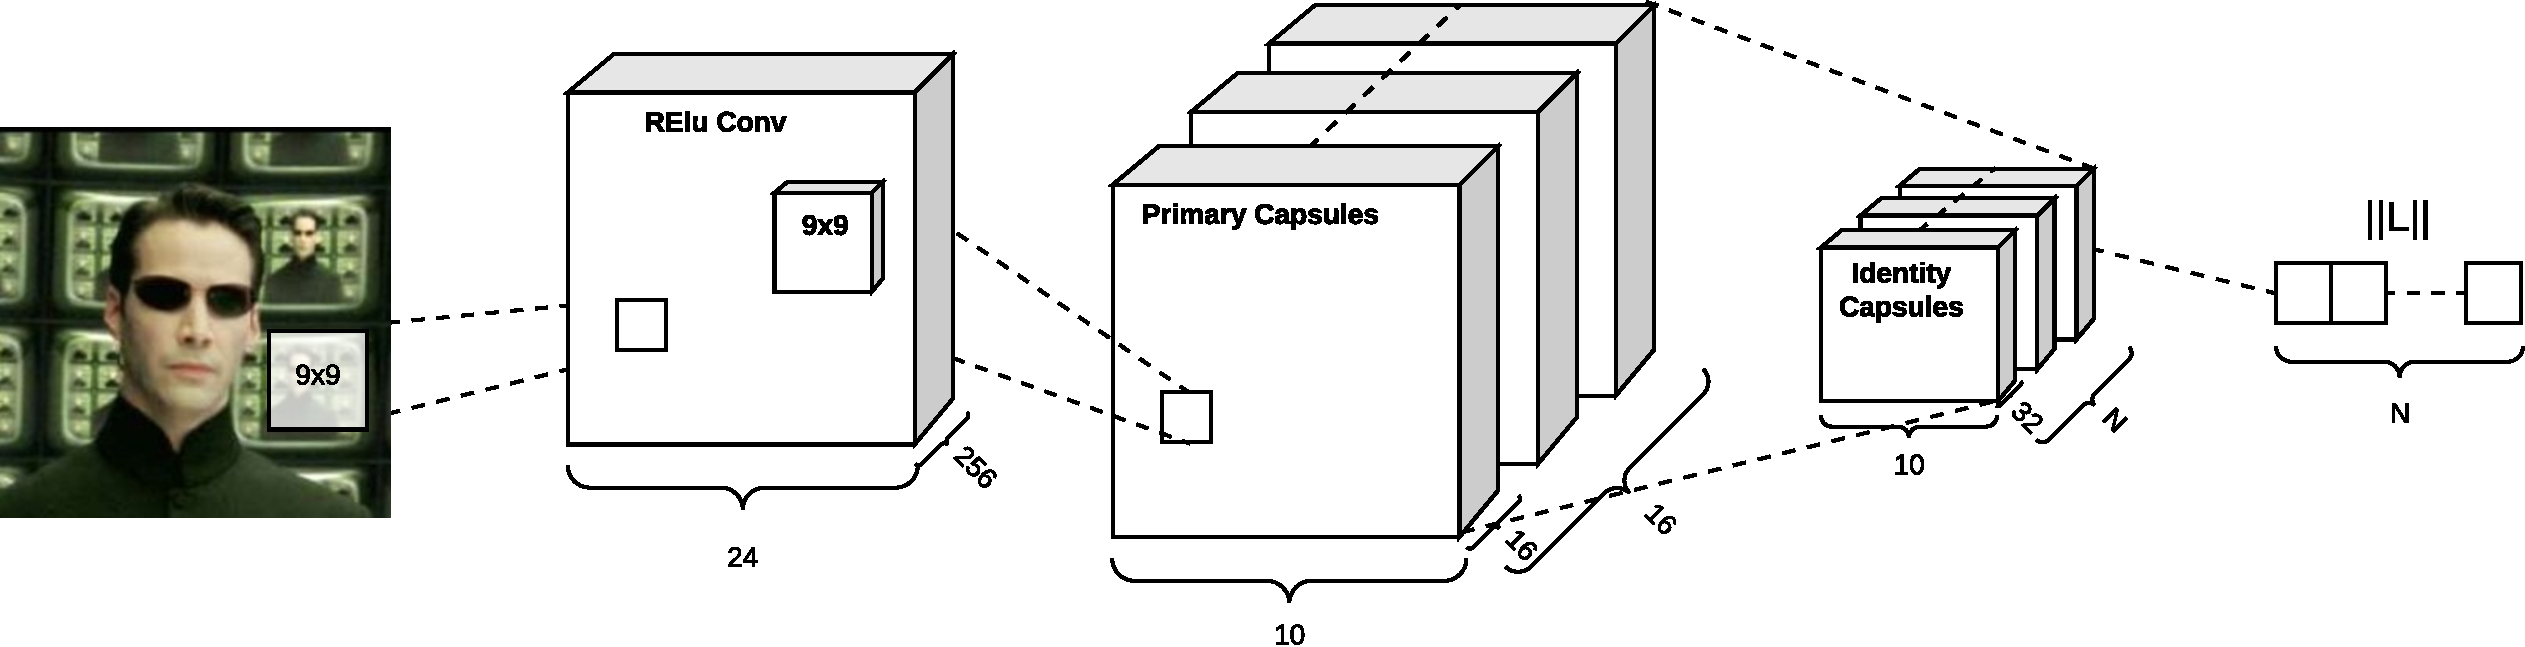
\includegraphics[width=\textwidth]{obrazky-figures/my_capsnet_encoder.pdf}
    \caption{Encoder visualization}
    \label{fig:my_encoder}
\end{figure}

\begin{enumerate}
    \item Input image is consumed as a
    \item Then standard 2D convolution is applied
    \item Convoluted output is routed towards the primary, feature capsules
    \item Prediction capsules measures activation on the previous layer and provides a weight based decision of likelihood that the capsule label matches the input.
\end{enumerate}

Additionally we add a \textit{Dropout} layer in between step 1 and 2 to prevent over-fitting on over-represented labels.

As you can see, the network itself is not complicated much. Let's take look at the implementation itself:

\begin{lstlisting}[language=Python, caption=Features capsule with squash activation]
x = layers.Input(name='input_image', shape=input_shape)

conv = layers.Conv2D(
    filters=init_conv_filters,
    kernel_size=init_conv_kernel,
    strides=1,
    padding='valid',
    activation='relu',
    name='encoder_conv2d'
)(x)

dropout = layers.Dropout(.3, name='encoder_dropout')(conv)

feature_caps = FeatureCapsule(
    capsule_dim=feature_caps_dim,
    channels_count=feature_caps_channels,
    kernel_size=feature_caps_kernel,
    strides=2,
    padding='valid',
    name='encoder_feature_caps'
)(dropout)

prediction_caps = PredictionCapsule(
    capsule_count=bins,
    capsule_dim=prediction_caps_dim,
    routing_iters=routing_iters,
    kernel_initializer=kernel_initializer,
    name='encoder_pred_caps'
)(feature_caps)

output = layers.Lambda(
    length,
    name='capsnet'
)(prediction_caps)
\end{lstlisting}

As you can see the implementation is quite versatile and allows a lot possibilities to configure and tune it's behavior. We have available quite few adjustable parameters and some more dependent on circumstances in which the model is deployed. We can convey the later group first and then provide explanation of the tunable parameters.

\begin{itemize}
    \item \texttt{input\_shape} is an essential attribute based on the input data. It allows the network to be prepared for input images of certain height and width. Multiple layers are directly or indirectly dependent on proper settings of this size.
    \item \texttt{bins} Allows researcher to set the amount of identities which we want to classify. This should also be dependent on the input data, since setting this value to different amount might result in false positive identifications.
\end{itemize}

Now to the more interesting arguments, which doesn't affect the model boundaries, but rather focus on performance and accuracy. It's worth mentioning that any of these arguments has impact on the architecture and model size, since they will change the number of trainable parameters.

\begin{itemize}
    \item \texttt{init\_conv\_filters} sets how many different features should be detected in the very first convolution layer.
    \item \texttt{init\_conv\_kernel} modifies the 2D dimensions of the kernel used in the first convolution layer.
    \item \texttt{feature\_caps\_kernel} is used to adjust the dimensions of convolutional kernel in the \textit{Primary feature capsules}.
    \item \texttt{feature\_caps\_dim} defines dimensionality of a capsule in the \textit{Primary feature capsules} layer.
    \item \texttt{feature\_caps\_channels} is another attribute of the \textit{Primary feature capsules}, which signifies amount of channels from which each capsule should build its grid of feature
    \item \texttt{prediction\_caps\_dim} sets the dimensionality of each capsule in \textit{Prediction capsules} layer. This effect the amount of features which are accented - sets the maximum connection limit for each prediction capsule towards the feature capsules.
    \item \texttt{kernel\_initializer} specifies the weight initialization in \textit{Prediction capsules}.
    \item \texttt{routing\_iters} allows a user to select the amount of iterations the dynamic routing should take.
\end{itemize}

Now once the scheme in general has been communicated, it's obvious that key knowledge is hidden in the implementation of the capsule layers. That would also provide explanation to the parameters mentioned above and their importance.

\subsection{Primary feature capsules layer}

Name of this layer and expectations set by previous chapters promise that great deal of invention is present n this layer. However that's not entirely true. More interesting behavior can be found in the next prediction capsules layer. The primary capsules are designed for a simple feature extraction as it might be known from traditional convolutional networks. This feature extraction has a twist to it, though. As prescribed in the chapter \ref{chapter:research}, a non linear \textit{squash} activation is used here. We've already conveyed the equation \ref{eq:squash} describing the real nature of the squash function. Now we have the opportunity to cover this in a code.

The feature capsules layer is in it's true nature a composite layer of three layers stacked and with the squash activation on output.

\begin{enumerate}
    \item At first a convolutional layer is present. This ensures extraction of multiple interesting patterns from each image. Patterns like hue, edges, orientation, dark spots etc. are recognized and represented by their belonging kernels. The amount of kernels corresponds to number of desired patters and dimensionality of each capsule.
    \item As a next step the convoluted vector is reshaped to be bundled by capsule dimensionality. This essentially splits the input tensor into separate capsules.
    \item And as the last step the \textit{squash} activation is used to provide non-linear normalization of each vector.
\end{enumerate}


\begin{lstlisting}[language=Python, caption=Features capsule with squash activation]
def squash(inputs, axis=-1):
    inputs += k.epsilon()   # Avoid ZeroDivisionError
    s_norm = k.sum(k.square(inputs), axis, keepdims=True)
    scale = s_norm / (1 + s_norm) / k.sqrt(s_norm)
    return scale * inputs

# Locate features
layers.Conv2D(
    capsule_dim*channels_count,
    kernel_size,
    strides=strides,
    padding=padding,
    name='feature_capsules_conv2d'
)(inputs)

# Split into capsules (concatenate kernels for each)
outputs = layers.Reshape(
    [-1, capsule_dim],
    name='feature_capsules_reshape'
)(outputs)

# Normalize
outputs = layers.Lambda(
    squash,
    name='feature_capsules_squash'
)(outputs)

# Result tensor
output
\end{lstlisting}

As you might see, there's nothing really complex happening in this layer. However when this layer is connected to prediction capsules, interesting things will start happening to properly determine the proper bond between capsules.

\subsection{Prediction capsules layer}

In Hinton's \cite{capsule} architecture suggestion, this is the final capsule layer. Intention is to classify feature capsule activations and provide routes to data from interesting feature capsules
for each particular label. As this might suggest, each prediction capsule is tightly mapped and bonded to a specific label. Therefore as much labels the network aims to classify, that much prediction capsules it has to contain. This is for sure a great scaling set back and this and few other drawbacks will be discussed as a part of our conclusion. For now, let's focus on how this capsule type is implemented and how we deal with the dynamic routing as described in chapter \ref{chapter:research}.

There are few shared properties in this layer. These are:

\begin{itemize}
    \item \texttt{capsule\_count} is a mandatory argument responsible for setting th amount of capsules available in this layer. This number corresponds to the labels we want the network to classify to.
    \item \texttt{capsule\_dim} is a second mandatory parameter defining dimensionality of each capsule. Recommended settings is 32 or greater. Increasing any of these two parameters has a great impact on size of the network.
    \item \texttt{kernel\_initializer} provides a string pointer or a object from \texttt{keras.initializers}. This parameter allows user to define initial values of capsule's weight matrices.
    \item \texttt{routing\_iters} allows to change and experiment with the amount of iterations of \textit{dynamic routing}. Default value is 3, although the best value may differ.
\end{itemize}

\begin{table}[ht]
    \centering
    \begin{tabularx}{.8\textwidth}{l|X}
        \toprule
        Count of capsules & \texttt{capsule\_count} \\
        Dimensionality of each capsule & \texttt{capsule\_dim} \\
        Amount of routing iterations & \texttt{routing\_iters} \\
        Count of input layer capsules (feature capsules) & \texttt{input\_capsule\_count} \\
        Dimensionality of input layer capsules & \texttt{input\_capsule\_dim} \\
        Weight matrix & \texttt{W} \\
        \bottomrule
    \end{tabularx}
    \caption{Prediction capsule layer attributes}
\end{table}

These are the building blocks and a complete context boundaries in which a prediction capsule is defined.

\begin{enumerate}
    \item Let's assume we have the input shape for this layer as \texttt{(None, input\_capsule\_count, input\_capsule\_dim)}.
    \item To allow space for manipulation in the prediction capsule space, we need to inject a new dimension into the input tensor and tile the \texttt{capsule\_count} over it. That way we can achieve a separate set of the initial input for a capsule in the current layer. Now we have shape \texttt{(None, capsule\_count, input\_capsule\_count, input\_capsule\_dim)}.
    \item Implementing the operation described in equation \ref{eq:capsule} we multiply the weight matrix \texttt{W}
\end{enumerate}

Now, once more in code:

\begin{lstlisting}[language=Python, caption=Prediction capsule call without routing]
# Prepare inputs
# inputs == [None, input_capsule_count, input_capsule_dim]
u = k.expand_dims(inputs, 1)
# u == [None, 1, input_capsule_count, input_capsule_dim]
u = k.tile(u, (1, capsule_count, 1, 1))
# u == [None, capsule_count, input_capsule_count, input_capsule_dim]

# Perform: inputs x W by scanning on input[0]
u = tf.einsum('iabc,abdc->iabd', u, W)
# u == [None, capsule_count, input_capsule_count, capsule_dim]
\end{lstlisting}

After the initial weight propagation is done, proper activation has to be ensured. Therefore using the dynamic routing is essential. This procedure was already described as Algorithm\,\ref{alg:routing}, however implementation-wise in \textit{Keras} it would look more like this:

\begin{lstlisting}[language=Python, caption=Prediction capsule routing]
# Init log prior probabilities to zeros:
b = tf.zeros(
    shape=(k.shape(inputs)[0], capsule_count, input_capsule_count, 1)
)
# b == [None, capsule_count, input_capsule_count, 1]

for i in range(routing_iters):
    with tf.variable_scope(f'routing_{i}'):
        c = tf.keras.activations.softmax(b, axis=1)
        # c == [None, capsule_count, input_capsule_count, 1]
        # Perform: sum(c x u)
        #
        # c == [None, capsule_count, input_capsule_count, 1]
        # u == [None, capsule_count, input_capsule_count, capsule_dim]
        s = tf.reduce_sum(tf.multiply(c, u), axis=2, keepdims=True)
        # s == [None, capsule_count, 1, capsule_dim]
        # Perform: squash
        v = squash(s)
        # v == [None, capsule_count, 1, capsule_dim]

        # Perform: sum(output x input)
        v_tiled = tf.tile(v, (1, 1, input_capsule_count, 1))
        b += tf.reduce_sum(
            tf.matmul(u, v_tiled, transpose_b=True),
            axis=3, keepdims=True
        )
        # b == [None, capsule_count, input_capsule_count, 1]

# Squeeze the extra dim (used for manipulation, not needed on output)
# v == [None, capsule_count, 1, capsule_dim]
v = tf.squeeze(v, axis=2)
# v == [None, capsule_count, capsule_dim]
\end{lstlisting}

The routing eliminates the \texttt{input\_capsule\_count} and \texttt{input\_capsule\_dim} from the tensor and instead provides new dimension of \texttt{capsule\_dim} which applies the attribute of current prediction capsule layer. As you can see the resulting shape of a prediction capsule classification activations per each image over each capsule dimension is the proper output shape of the layer. This would eventually tell us, which capsule found that particular image most interesting and the likelihood that it belongs to a class mapped to a capsule.

\section{Decoder}

Based on the findings in Chapter\,\ref{chapter:research}, a decoder is a sequential model meant to provide an image reconstruction feedback. The gro is to implement a training helper, which covers the key spatial feature areas of a particular identity, so we can later compare and match the input image to measure accuracy of our prediction. In case of a MNIST data-set this factor is of a great help, though in case of coherent input data with small difference on large spatial feature scale, as a human face image is, the importance of a decoder seems diminished. Moreover a simple 3 layers deep decoder comprising of fully connected layers offered by research on MNIST can't be successfully used on RGB data with granular features. Therefore we leverage a solution introduced by Thibault Neveu in his traffic signs classifier\,\ref{ss:traffic_signs}. We will build a convoluted reconstruction model, which essential building blocks are a dense layer, resizing layers and convolutional layers. In the end this forms a neural network of 10 layers, which provides more detail than a 3 layer model of fully connected layers.

The decoder consumes a prediction provided by \textit{encoder} as well as the true image and aims to recreate a image of a face based on the feature grid activations in the prediction. The result can be understood as a master template for that particular identity. We will look into that in our model evaluation later.

Now, let's describe the flow we want the layers to convey in our decoder unit:

\begin{enumerate}
    \item \texttt{keras.layers.Dense} which normalizes and unifies the input mapping enabling later convolutions to run efficiently and select proper input activations.
    \item \texttt{keras.layers.Reshape} layer converts the fully connected output from one dimensional array to a base image matrix with $5\times5$ pixels over 16 channels.
    \item Now an alternating pattern of \texttt{keras.layers.Conv2D} and \texttt{keras.layers.Lambda} with \texttt{resize} function provides a resizing, up-scaling of the image, while interpolating its properties back to $32\times32$ pixels in a convoluted fashion.
    \item Before we finalize the decoder, another \texttt{keras.layers.Conv2D} convolutional layer is used to reduce populated channels and provide only one best channel for each colour.
    \item As the last layer we chose to chain an activation layer \texttt{keras.layers.Activation} transforming our matrices to a ReLU activated image data.
\end{enumerate}

In case this is not explanatory enough, let's look at a diagram:

\begin{figure}[ht]
    \centering
    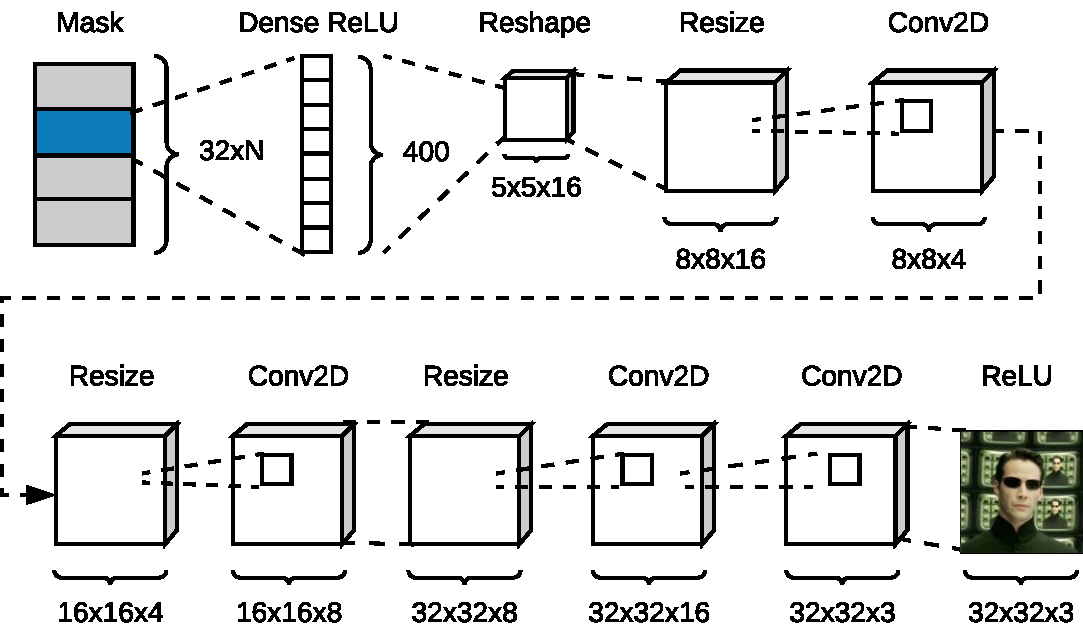
\includegraphics[height=18em]{obrazky-figures/my_decoder.pdf}
    \caption{A convolutional decoder for a \textit{CapsNet} used in our implementation.}
    \label{fig:decoder}
\end{figure}

\subsection{Masking layer}

Since we want our \textit{decoder} to provide as accurate reconstruction we need tell it, when the predicted output matches our expectation on what capsule. So before we pass our \textit{encoder} output to the \textit{decoder} defined above, we need to build a mechanism which would combine true labels and predicted activations in our capsules. This can be easily done by introducing an intermediate layer, which can nullify every other capsule vector than the correct one. And since we already have our labels defined as a hot one encoding, we can just simply multiply our capsule network encoder findings as a tensor for each input by the label vector. That will ensure propagation of correct capsule activations, because they happen to be on the only (hot) index, while other capsules are deactivated because their vector is multiplied by a zero, therefore they won't provide any input value for this image. Therefore we end up with set of vectors per each label in size of $\texttt{capsule\_dim}\times\texttt{labels\_count}$. Despite we consume two outputs in this layer, the output shape can be computed solely from the first input\,--\,the \textit{prediction capsule} layer shape. The dimension of true labels is shared because we keep the number of identities and amount of capsules consistent (1 to 1 mapping).

\begin{figure}[ht]
    \centering
    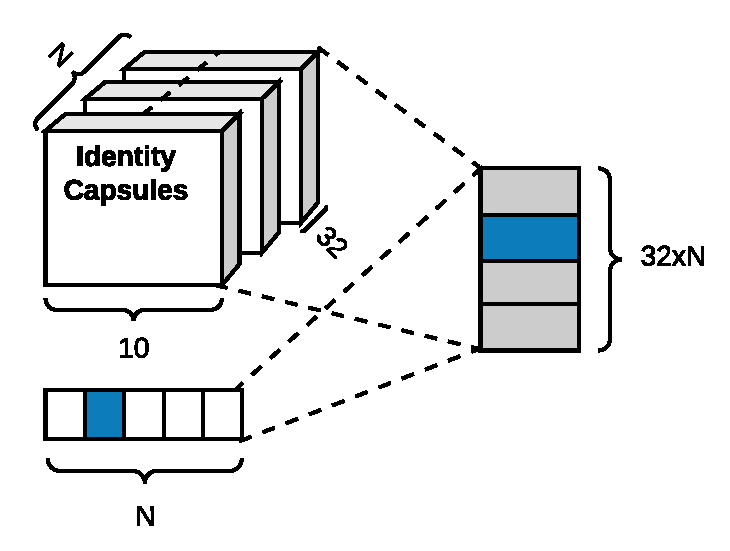
\includegraphics[height=14em]{obrazky-figures/my_mask.pdf}
    \caption{Graphical representation of the masking layer. Colo coded in blue is the reconstruction target, while in gray are the suppressed inputs.}
    \label{fig:mask}
\end{figure}

This layer is straightforward to implement. Despite the simple calculation, it would be difficult to use \texttt{keras.layers.Lambda} since we are combining 2 inputs and calculating the output shape out of them, therefore we take the base \texttt{keras.layers.Layer} and extend it's \texttt{call} and \texttt{compute\_output\_shape} methods. Since this layer doesn't require trainable weights, there's no need to overwrite the default \texttt{\_\_init\_\_} on \texttt{build}.

\begin{lstlisting}[language=Python, caption=Masking layer]
class Mask(layers.Layer):
    def call(self, inputs, **kwargs):
        # Unpack
        capsule_output, labels = inputs
        # A vector is multiplied by a scalar hot one encoding.
        # Therefore only one vector is kept.
        return k.batch_flatten(capsule_output * k.expand_dims(labels))

    def compute_output_shape(self, input_shape):
        # PredictionCapsule layer shape
        # input_shape[0].shape == (None, capsule_count, capsule_dim)

        # True labels shape
        # input_shape[1].shape == (None, capsule_count)

        # Calculate from PredictionCapsule shape
        return (None, input_shape[0][1] * input_shape[0][2])
\end{lstlisting}


\subsection{Recapitulation}

Now we understand the building blocks of our network. Let's recapitulate the whole architecture to better understand the complete flow how the data will be processed and classified. We begin with an image of a human face. This image is set to be $32\times32$ pixels and the ground truth labels are expected to be a hot one encoding of the vectorized identity bins.

Then we can expect the \textit{encoder} to adhere to the architecture shown on Fig\,\ref{fig:my_encoder}. When the model is validated or we are running an inference, we just calculate a norm by length over the outputs are we have a prediction. On the other hand, when the model is being trained, we need to add a \textit{decoder}. However, in between we can't forget about the intermediate layer encoding the true labels for reconstruction. So we plug there the \textit{masking layer}, after which we can successfully chain the \textit{decoder}. Let's have a look how a summary of such model would look like:

\begin{table}[ht]
    \centering
    \resizebox{\linewidth}{!}{
        \begin{tabular}{l|l|l|r|l}
            \toprule
            Name                                     & Type                       & Output shape          & Parameters     & Connected to\\
            \midrule
            \texttt{input\_image}                    & \texttt{Input}             & $(None, 32, 32, 3)$   & \num{0}        & \\
            \texttt{encoder\_conv2d}                 & \texttt{Conv2D}            & $(None, 24, 24, 512)$ & \num{124928}   & \texttt{input\_image}\\
            \texttt{encoder\_dropout}                & \texttt{Dropout}           & $(None, 24, 24, 512)$ & \num{0}        & \texttt{encoder\_conv2d}\\
            \texttt{encoder\_feature\_caps\_conv2d}  & \texttt{Conv2D}            & $(None, 10, 10, 256)$ & \num{3277056}  & \texttt{encoder\_dropout}\\
            \texttt{encoder\_feature\_caps\_reshape} & \texttt{Reshape}           & $(None, 1600, 16)$    & \num{0}        & \texttt{encoder\_feature\_caps\_conv2d}\\
            \texttt{encoder\_feature\_caps\_squash}  & \texttt{Lambda (squash)}   & $(None, 1600, 16)$    & \num{0}        & \texttt{encoder\_feature\_caps\_reshape}\\
            \texttt{encoder\_pred\_caps}             & \texttt{PredictionCapsule} & $(None, 42, 32)$      & \num{34406400} & \texttt{encoder\_feature\_caps\_squash}\\
            \texttt{capsnet}                         & \texttt{Lambda (length)}   & $(None, 42)$          & \num{0}        & \texttt{encoder\_pred\_caps}\\
            \texttt{input\_label}                    & \texttt{Input}             & $(None, 42)$          & \num{0}        & \\
            \texttt{mask}                            & \texttt{Mask}              & $(None, 1344)$        & \num{0}        & \texttt{encoder\_pred\_caps}\\
                                                     &                            &                       &                & \texttt{input\_label}\\
            \texttt{decoder\_dense}                  & \texttt{Dense}             & $(None, 400)$         & \num{538000}   & \texttt{mask}\\
            \texttt{decoder\_reshape\_1}             & \texttt{Reshape}           & $(None, 5, 5, 16)$    & \num{0}        & \texttt{decoder\_dense}\\
            \texttt{decoder\_resize\_1}              & \texttt{Lambda (resize)}   & $(None, 8, 8, 16)$    & \num{0}        & \texttt{decoder\_reshape\_1}\\
            \texttt{decoder\_conv2d\_1}              & \texttt{Conv2D}            & $(None, 8, 8, 4)$     & \num{580}      & \texttt{decoder\_resize\_1}\\
            \texttt{decoder\_resize\_2}              & \texttt{Lambda (resize)}   & $(None, 16, 16, 4)$   & \num{0}        & \texttt{decoder\_conv2d\_1}\\
            \texttt{decoder\_conv2d\_2}              & \texttt{Conv2D}            & $(None, 16, 16, 8)$   & \num{296}      & \texttt{decoder\_resize\_2}\\
            \texttt{decoder\_resize\_3}              & \texttt{Lambda (resize)}   & $(None, 32, 32, 8)$   & \num{0}        & \texttt{decoder\_conv2d\_2}\\
            \texttt{decoder\_conv2d\_3}              & \texttt{Conv2D}            & $(None, 32, 32, 16)$  & \num{1168}     & \texttt{decoder\_resize\_3}\\
            \texttt{decoder\_conv2d\_4}              & \texttt{Conv2D}            & $(None, 32, 32, 3)$   & \num{435}      & \texttt{decoder\_conv2d\_3}\\
            \texttt{decoder\_activation}             & \texttt{Activation}        & $(None, 32, 32, 3)$   & \num{0}        & \texttt{decoder\_conv2d\_4}\\
            \midrule
            \multicolumn{3}{l|}{Total}                                                                    & \num{38348863} & \\
            \bottomrule
        \end{tabular}
    }
    \caption{Implemented CapsNet architecture: Each model in different conditions can differ in number of parameters and and each layer shapes. For example initial convolution can be set to different amount of filters which is determined by experiment. Other example can be the amount of capsules in prediction layer (and its output shape) since that is tightly bonded to the amount of identity bins. Listed layer types are understood to belong to \texttt{keras.layers} namespace. In case of \texttt{Lambda} layers, the function in use is listed in parenthesis.}
\end{table}

\section{Life cycle of a model}

Traditionally in machine learning a model needs to be trained, then it is tested and validated. Since there's no reason to change this workflow this section will follow the established scheme and walk you through the required steps in the particular order in which they need to be examined:

\begin{enumerate}
    \item Data set selection, collection and pre-processing
    \item Establishing model
    \item Training a model
    \item Validation of trained accuracy
    \item Publishing results
\end{enumerate}

\subsection{Data set preparation}

In previous chapters suitable data sets were already mentioned and elaborated. Since size of our solution is greatly dependent on the amount of identities, we need to select a data set with fair ratio between the size of labels vector and amount of samples per each identity. For this particular demonstration we chose the \textit{Labeled Faces in the Wild}\,\ref{ss:lfw} due to fair distribution when limited to 25 samples per label or greater, and its simplicity to collect via \textit{scikit-learn}\footnote{\url{https://scikit-learn.org}} library. We also tried and demonstrated in our Jupyter notebooks the \textit{PINS}\,\ref{ss:pins} data set, but the diversity in data proved itself to be of no use. However the collection code remains in the thesis sources and in the notebooks, so it is available to be experimented with.

For next parts of this text, we will continue to use the \textit{LFW} data set as the sole example for input data. In order to collect this data set we don't need to be inventing the wheel again and we can leverage the capabilities granted via \texttt{sklearn} library.

\begin{lstlisting}[language=Python, caption=Collect Labeled Faces in the Wild data set]
people = fetch_lfw_people(
    color=True,
    min_faces_per_person=25,
)
\end{lstlisting}

By default the images are $300\times300$ pixels big, though since we aim to process images as small as $32\times32$ pixels we need to resize the images. We can either try to reason with a \texttt{resize=} parameter, though this size fraction can prove itself unreliable so we will use help of the \textit{Pillow}\footnote{\url{https://pillow.readthedocs.io}} library:

\begin{lstlisting}[language=Python, caption=Pre-processing of the data set]
x = people.images

def downsample(image):
    image = Image.fromarray(image.astype('uint8'), 'RGB')
    image = image.resize(resize_to, Image.ANTIALIAS)

    return np.array(image)

x = np.array([downsample(i) for i in x]) / 255
\end{lstlisting}

Now we have solved the image sizes, we can prepare the data set into two distinct bundles, one for training and one for validation. This means the data we are training the model against are not the same we use later for validation, therefore the result of validation is pure and not affected by over-fitting. Here we can use the help of \textit{scikit-learn} library once again, since it provides a \texttt{train\_test\_split} function which allow us to separate these two sets randomly, with a respective desired ratio. And last but not least, we need to convert our labels to a hot one encoding. This time we can use a \textit{Keras} native function \texttt{to\_categorical}.

The data set is now prepared, let's take a look at the distribution of images magnitude per label that we can expect as well as other metrics we may consider before training. As we can see on following Fig\,\ref{fig:lfw_distribution}, the distribution is not ideal, and our model will have a tendency to over-fit on certain overrepresented labels and under-fit on others. This is unfortunate and we can try to eliminate such behavior by a \textit{dropout} layer and with additional augmentation.

\begin{figure}[ht]
    \centering
    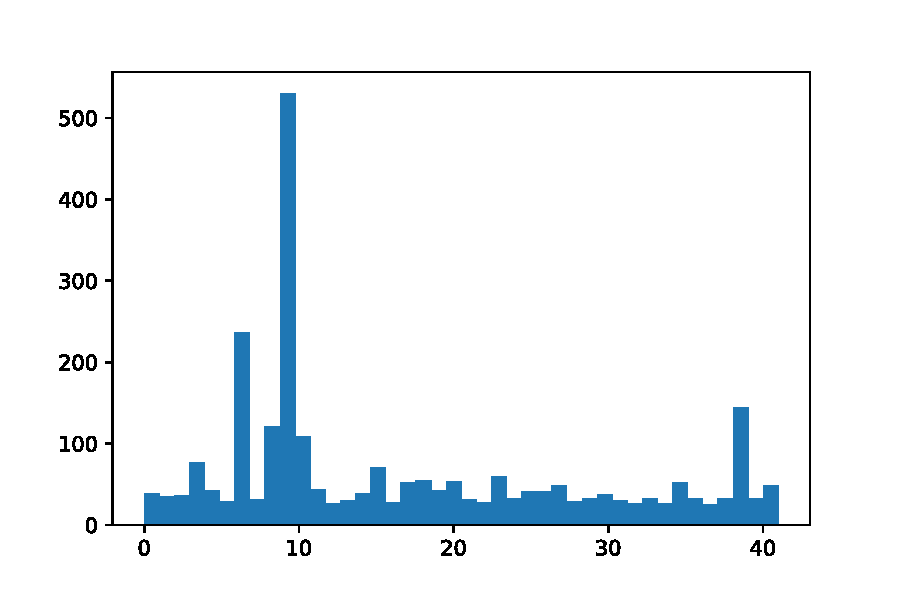
\includegraphics[height=14em]{obrazky-figures/lfw_distribution.pdf}
    \caption{LFW subset distribution}
    \label{fig:lfw_distribution}
\end{figure}

\begin{table}[ht]
    \centering
    \begin{tabularx}{.8\textwidth}{l|X}
        \toprule
        Number of subjects & \num{42} \\
        Total amount images & \num{2588} \\
        Amount of images for \textbf{training} & \num{2070} \\
        Amount of images for \textbf{testing} & \num{518} \\
        Minimum samples per subject & \num{25} \\
        Maximum samples per subject & \num{521} \\
        Resolution & $32\times32$ px \\
        Channels & 3 color channels, RGB \\
        \bottomrule
    \end{tabularx}
    \caption{Metrics of the used subset of \textit{LFW} data set}
\end{table}

\subsection{Train}

Training of a \textit{Keras} model can be handled in multiple different ways. Since our model requires multiple input and provides multiple outputs when trained, the \texttt{fit\_generator} approach was used. It provides greater control over data passed to the model than a simple \texttt{fit}, while it remains a pretty simple to implement than a fully custom training. Naturally, the first and foremost in \textit{Keras}, we need to compile a model, then we can use the already mentioned \texttt{fit\_generator} method with a data generator to process the training.


\begin{lstlisting}[language=Python, caption=Training a \textit{Keras} mode using \texttt{fit\_generator}]
model.compile(
    optimizer=optimizers.Adam(lr=lr),
    loss=[margin_loss, 'mse'],
    loss_weights=[1., decoder_loss_weight],
    metrics={'capsnet': 'accuracy'}
)

history = model.fit_generator(
    generator=dataset_gen(x_train, y_train, batch_size=batch_size),
    steps_per_epoch=len(x_train) / batch_size,
    epochs=epochs,
    validation_data=[[x_test, y_test], [y_test, x_test]],
    verbose=1,
    callbacks=cb
)
\end{lstlisting}

As you may have noticed, you can see that we've used \texttt{keras.optimizers.Adam} optimizer and allow to configure the learning rate (\texttt{lr}), weight of the decoder loss function (\texttt{decorator\_loss\_weight}) as well as a batch size (\texttt{batch\_size}) and final amount of epochs. The training uses the margin loss function according to Eq.\,\ref{eq:margin_loss} and a data generator \texttt{dataset\_gen}. This generator provides additional data augmentation via standard \textit{Keras} image processors and yields two sets of data, one for each input with their respective validation truths:

\begin{lstlisting}[language=Python, caption=Data generator example]
def dataset_gen(x, y, batch_size):
    datagen = ImageDataGenerator(
        width_shift_range=0.1,
        height_shift_range=0.1,
        rotation_range=20,
        # horizontal_flip=True
    )
    generator = datagen.flow(x, y, batch_size=batch_size)
    while 1:
        x_batch, y_batch = generator.next()
        yield ([x_batch, y_batch], [y_batch, x_batch])
\end{lstlisting}

\subsection{Test model and predict labels}

Testing and providing predictions is a simple process, since everything comes already prepared with \textit{Keras} models. For testing purposes a model is required to be compiled, otherwise it can't provide loss calculations and therefore it can be tested. On the other hand, when we desire simple predictions the model doesn't need to be compiled, only presence of weights is required.

\begin{lstlisting}[language=Python, caption=Test run of a \textit{Keras} model example]
def test(model, x_test, y_test, batch_size=10):
    model.compile(
        optimizer='adam',
        loss=margin_loss,
        metrics={'capsnet': 'accuracy'}
    )
    return model.evaluate(x_test, y_test, batch_size=batch_size)
\end{lstlisting}

\begin{lstlisting}[language=Python, caption=Prediction example for a given model]
def predict(model, x, batch_size=10):
    return model.predict(x, batch_size=batch_size)
\end{lstlisting}

\subsection{Save and load a model}
\label{ss:save_model}

This is a last part of a model life cycle. Previous text showed how each phase contributes to creation of a model which finally allows a researched to observe and measure their experiments. To have a model last, we need a meaning to store it's trained properties as well as layout. Since our models allow great customization and invasive changes in the core architecture, we are obliged to persist not only the weight of every trainable parameter, but also a configuration of each layer, amounts of neurons in each, probability rates preset before even any training begun. \textit{Keras} library provides a mean how to achieve that. Each model can be transformed into a H5, JSON or YAML format, while only the H5 format allows us to save weights along with it. However, since the \textit{CapsNet} model is not a single model and we define two different models, one for training and one for inference, we have to keep our weights separate. Hence we save them as a H5 file separately and then proceed to store the model architectural configuration settings as a separate YAML file for each model. And just to keep everything together and bundled, we pack these 3 files into a gun-zipped tarball. This is how we can do it:

\begin{lstlisting}[language=Python, caption=Saving a model in \textit{Keras}]
with open('train.yml', 'w') as f:
    f.write(training_model.to_yaml())

with open('test.yml', 'w') as f:
    f.write(testing_model.to_yaml())

training_model.save_weights('weights.h5')
\end{lstlisting}

The process shown here is significantly simplified, since our tarball scenario requires more complex handling, but the principles stays the same. A similar process, yet reversed procedure can be used later to load the data back into a model instance. The implementation provided with this thesis allows passing a special parameter to \texttt{CapsNet} constructor which would skip the network initialization phase and allow to create a model from a class method. This \texttt{load} method uses native function \texttt{model\_from\_yaml} to load up the network configurations and later \texttt{load\_weights} methods to upload trained values. Since we store the weights from the more complex model only, the simplified testing model, is required to load the weights by layer name. Here is how it might look like in a simplified scenario. If a reader is interested in more details of this process, feel free to consult our sources.


\begin{lstlisting}[language=Python, caption=Loading a model in \textit{Keras}]
custom_objects = {
    # Custom layers unknown to Keras
    'PredictionCapsule': PredictionCapsule,
    'FeatureCapsule': FeatureCapsule,
    'Mask': Mask,
    # TensorFlow and Keras back-end functions used in lambda layers
    'tf': tf,
    'k': k
}

with open('train.yml', 'r') as f:
    training_model.model_from_yaml(f.read(), custom_objects=custom_objects)
training_model.load_weights('weights.h5')

with open('test.yml', 'r') as f:
    testing_model.model_from_yaml(f.read(), custom_objects=custom_objects)
testing_model.load_weights('weights.h5', by_name=True)
\end{lstlisting}

\section{Experiment}

Based on previous sections we have prepared our network to be successfully trained.
